\documentclass[11pt]{article}

\usepackage[margin=1in]{geometry}
\usepackage{amsmath}
\usepackage{amssymb}
\usepackage[T1]{fontenc}
\usepackage{textcomp}
\usepackage{booktabs}
\usepackage{graphicx}
\usepackage{hyperref}
\usepackage{parskip}

\newcommand{\uu}{\mathbf{u}}
\newcommand{\KK}{\mathbf{K}}
\newcommand{\CC}{\mathbf{C}}
\newcommand{\dK}{\delta\KK}
\newcommand{\code}[1]{\texttt{#1}}

\title{Comparing the motions of a protein and its mutants}
\author{Notes for penm}
\date{2026-10-16}

\begin{document}

\maketitle

\section{Scope}

These notes collect a review of penm's \code{delta\_motion\_*} measures, the measures
used in the literature on comparing protein motions, and a study of how a protein's normal
modes change under single-point mutations.
Everything numerical was computed with the scripts in this folder; each script's printed
output is saved beside it as \code{<script>.out.txt}.
The protein is 2acy throughout, and the results come from one protein, one model and one
ensemble: whether they generalise is not known.

\section{The motion measures in penm}

Let $\lambda_n,\uu_n$ be the eigenvalues and eigenvectors of the wild type's network matrix
$\KK$ over its $3N-6$ internal modes, $\mu_m,\mathbf{w}_m$ those of the mutant,
$\CC=\beta^{-1}\KK^{+}$ the covariance, $\sigma_n^2 = 1/(\beta\lambda_n)$, and
$O_{nm}=\uu_n\cdot\mathbf{w}_m$ the overlap matrix.
$\CC_{ii}$ is the $3\times3$ diagonal block of site $i$.

\begin{center}
\begin{tabular}{lp{9.2cm}l}
\toprule
function & quantity & depends on \\
\midrule
\code{dmsfi} & $\operatorname{tr}\CC^{\rm mut}_{ii}-\operatorname{tr}\CC^{\rm wt}_{ii}$ & site marginals \\
\code{dbhati} & Bhattacharyya distance between the zero-mean Gaussians with $\CC^{\rm wt}_{ii}$, $\CC^{\rm mut}_{ii}$ & site marginals \\
\code{rwsipi} & RWSIP of $\CC^{\rm wt}_{ii}$ and $\CC^{\rm mut}_{ii}$ & site marginals \\
\code{dhi} & $\tfrac12\ln\det\CC^{\rm mut}_{ii}/\det\CC^{\rm wt}_{ii}$ & site marginals \\
\code{dmsfn} & $\uu_n^{T}\CC^{\rm mut}\uu_n-\sigma_n^2$ & wt modes \\
\code{dhn} & $\tfrac12\ln\bigl(\uu_n^{T}\CC^{\rm mut}\uu_n/\sigma_n^2\bigr)$ & wt modes \\
\code{rwsipn} & $\bigl(\sigma_n^2\sum_m\mu_m^{-1}\beta^{-1}O_{nm}^2\big/\sum_k\sigma_k^2\beta^{-1}\mu_k^{-1}\bigr)^{1/2}$ & both mode sets \\
\code{nhn} & $\exp\bigl(-\sum_m O_{nm}^2\ln O_{nm}^2\bigr)$ & both mode sets \\
\bottomrule
\end{tabular}
\end{center}

The four site measures use only the $3\times3$ diagonal blocks, the marginal distribution of
each site: none of them sees a change in the correlations between sites.

\subsection{Identities}

Checked on one genm mutant (site 11, letter 1; \code{motion\_identities.R}):

\begin{itemize}
\item $\code{dhn}_n = \tfrac12\ln(1+\code{dmsfn}_n/\sigma_n^2)$ exactly.
\item $\code{rwsipn}_n = \bigl(\sigma_n^2(\sigma_n^2+\code{dmsfn}_n)/\sum_k\sigma_k^2\mu_k'\bigr)^{1/2}$
  exactly, with $\mu_k'$ the mutant's variances paired with the wild type's by rank,
  because $\sum_m O_{nm}^2/(\beta\mu_m) = \uu_n^T\CC^{\rm mut}\uu_n$.
  Given the wild type, \code{dhn} and \code{rwsipn} carry the same information as \code{dmsfn}.
\item $\sum_n\code{dhn}_n = -0.099$, while the entropy change is
  $\Delta S/k = -0.189 = -\beta\,\code{ddg\_tds}$.
  The two differ by $\tfrac12\bigl(\sum_n\ln[\CC']_{nn}-\ln\det\CC'\bigr)\ge0$, the
  multi-information of the mutant's covariance $\CC'$ in the wild type's mode basis, so the
  \code{dhn} do not decompose the entropy change.
\item \code{rwsipi} ranges over 0.9996--1 for this mutant.
\end{itemize}

\section{Measures in the literature}

The papers are in \code{dev/docs/references/comparison}.
All compare homologous proteins, which needs alignment, a common structural core,
superposition and, usually, normalisation of the amplitudes; penm compares a protein with
mutants built in the same network, on the same sites.

\begin{itemize}
\item \textbf{Maguid et al.\ 2005} (Biophys.\ J.\ 89:3). GNM modes of 18 globins, restricted to
  gap-free positions; modes matched across proteins by permuting the columns of the overlap
  matrix to maximise its trace; representative modes by SVD; Pearson $r$ of B-factor profiles.
\item \textbf{Maguid et al.\ 2006} (J.\ Mol.\ Evol.\ 63:448). Spearman $\rho_B$ of experimental
  C$_\alpha$ B-factor profiles of homologous pairs, against random pairs, with RMSD and
  sequence identity.
\item \textbf{Maguid et al.\ 2008} (Gene 422:7). GNM. Mode conservation $S_{nn}$, the diagonal of
  the overlap matrix after reassignment; collectivity
  $\kappa_n = N^{-1}\exp(-\sum_i q_{in}^2\ln q_{in}^2)$; Spearman correlation of B-factor
  profiles. Conservation decreases with mode index and correlates with collectivity.
\item \textbf{Fuglebakk, Echave \& Reuter 2012} (Bioinformatics 28:2431). A score is a property
  ($\CC$, the correlation matrix $\mathbf{P}$, the isotropic $\CC_{\rm iso}$ and
  $\mathbf{P}_{\rm iso}$, the RMSF profile) and a measure (RMSIP over 10 modes, RWSIP, and a
  normalised Bhattacharyya distance NDB between zero-mean Gaussians after trace normalisation
  and projection onto a common subspace). Judged by agreement with SCOP: the property matters
  more than the measure; RMSF profiles do worst; NDB($\CC$) and RWSIP($\mathbf{P}$) do best,
  rivalling RMSD.
\item \textbf{Micheletti 2013} (Phys.\ Life Rev.\ 10:1, review). RMSIP; a per-residue profile
  $Q_i$ of it; the distance-weighted RMSIP of Zen et al.\ 2008, which combines structure and
  motion by weighting each aligned residue with
  $f(d_i)=[1-\tanh((d_i-4\,\text{\AA})/2\,\text{\AA})]/2$; matrices of distance fluctuations
  (M\"unz et al.).
\item \textbf{Echave 2013} (comment on the review). The low modes may be conserved because they
  are robust to random mutations, not because selection keeps them.
\item \textbf{Granata et al.\ 2017} (PNAS 114:E10612). Compares partitions into domains,
  coevolutionary against SPECTRUS dynamical domains, by adjusted mutual information.
\end{itemize}

The review describes Maguid et al.\ 2006 and 2008 as using an anisotropic ENM; the papers
themselves use experimental B-factors (2006) and the isotropic GNM (2008).

\section{Eigenvector and eigenvalue changes}

A mutation changes both the eigenvectors and the eigenvalues.
To first order in $\dK=\KK^{\rm mut}-\KK^{\rm wt}$,
\begin{equation}
\delta\lambda_n = \uu_n^T\dK\,\uu_n,
\qquad
c_{mn} = \frac{\uu_m^T\dK\,\uu_n}{\lambda_n-\lambda_m}\quad(m\neq n):
\end{equation}
eigenvalues respond to the diagonal of $\dK$ in the wild type's basis, eigenvectors to the
off-diagonal, divided by the gaps.

\paragraph{Eigenvectors.} \code{nhn} is the exponential of the entropy of the distribution
$O_{nm}^2$ of wild-type mode $n$ over the mutant's modes: the number of mutant modes it spreads
into. It needs no reassignment of modes.

\paragraph{Eigenvalues.} Comparing the sorted spectra, $\mu_n$ against $\lambda_n$, is itself an
assignment: it pairs modes by rank, which pairs different modes wherever they cross.
Only functions symmetric in the eigenvalues, such as $\sum_n\ln\lambda_n$ in \code{ddg\_tds},
are free of assignment. Two per-mode quantities are free of it:
\begin{align}
\uu_n^T\KK^{\rm mut}\uu_n &= \lambda_n + \delta K_{nn} = \textstyle\sum_m O_{nm}^2\mu_m, \\
\uu_n^T\CC^{\rm mut}\uu_n &= \textstyle\sum_m O_{nm}^2/(\beta\mu_m).
\end{align}
Both are Rayleigh quotients at the wild-type mode: the eigenvector change enters them at
second order. Their second-order contamination falls on opposite ends of the spectrum: the
$\CC$ form weights by $1/\mu$, so a small admixture of a soft mutant mode into a stiff wild-type
mode can dominate it; the $\KK$ form weights by $\mu$, the reverse. How large either effect is
on real mutants was not measured. \code{dmsfn} is the $\CC$ form minus $\sigma_n^2$.

If the springs are perturbed in proportion to their stiffness, $\delta k_{ij}=\epsilon_{ij}k_{ij}$
with mean $\bar\epsilon$, then $E[\delta\lambda_n]=\bar\epsilon\lambda_n$ to first order: the relative
change of the eigenvalues is the same for every mode, $\delta(1/\lambda)\propto1/\lambda$, and the low
modes change most in absolute fluctuation and equally in relative terms.

\paragraph{Close is not degenerate.} When $\lambda_n=\lambda_m$ exactly, the individual eigenvectors are
undefined within their subspace and their rotation has no physical meaning. When the eigenvalues are
close but distinct, the eigenvectors are defined but sensitive: a perturbation with
$|\delta K_{nm}|\gtrsim|\lambda_n-\lambda_m|$ rotates them, and the mutant's normal modes really are
different. Closeness is the gap measured against the perturbation, not a property of the spectrum
alone. When two close modes rotate within their span, the covariance changes little, by about the
gap times the rotation: the vibrational directions can change a lot while the fluctuations change
little. \code{nhn} measures the first; measures built on $\CC$ measure the second.

\section{A network and its complement}

For a graph Laplacian $\mathbf{L}$ (the GNM's Kirchhoff matrix), the complement graph's Laplacian is
$\bar{\mathbf{L}} = n\mathbf{I}-\mathbf{J}-\mathbf{L}$, with $\mathbf{J}$ the matrix of ones.
Both annihilate $\mathbf{1}$, so they commute, share eigenvectors, and $\bar{\mathbf{L}}\uu=(n-\lambda)\uu$
for $\uu\perp\mathbf{1}$: the complement's lowest modes are the graph's highest.
With weights, the same holds for complement weights $c-w_{ij}$.
On 2acy (\code{complement.R}, $d_{\max}=10.5$\,\AA): $\mathbf{L}+\bar{\mathbf{L}}=n\mathbf{I}-\mathbf{J}$,
the commutator is exactly zero, and the non-zero eigenvalues of $\bar{\mathbf{L}}$ are $n-\lambda$.

For the 3D Hessian of an ANM it fails: the complete network's Hessian has blocks
$\mathbf{e}_{ij}\mathbf{e}_{ij}^T$ that depend on the geometry and is not a multiple of a
projector. On 2acy the relative commutator $\|\mathbf{H}\bar{\mathbf{H}}-\bar{\mathbf{H}}\mathbf{H}\|/(\|\mathbf{H}\|\|\bar{\mathbf{H}}\|)$
is 0.017, and the best overlap of each mode of $\mathbf{H}$ with any mode of $\bar{\mathbf{H}}$ has median 0.22.

In the GNM, perturbing $G$ by $\delta$ is exactly perturbing $\bar G$ by $-\delta$, so the
robustness of mode $n$ of $G$ equals that of the mode at the opposite end of $\bar G$'s spectrum.
This is a symmetry between two graphs, not between the low and high modes of one graph: a
contact graph is sparse and its complement dense. What it does show is that low versus high is
not intrinsic to eigenvector stability, which depends on $|\lambda_n-\lambda_m|$ and $|\delta K_{nm}|$,
both unchanged by $\lambda\to c-\lambda$; the profile of robustness against $n$ must come from how gaps
and couplings are distributed over the spectrum.

\section{A mutational scan: is mean \code{nhn} explained by the spectral density?}

\paragraph{Setup.} The genm vignette's wild type: \code{node = "ca"}, \code{model = "ming\_wall"},
$d_{\max}=10.5$\,\AA, \code{d\_max\_graph = 14}, \code{ensemble = 1}, \code{alphabet\_size = 10},
\code{mut\_dl\_sigma = 0.3}, \code{mut\_sd\_min = 2}. All 882 single-point mutants (98 sites,
9 letters each; \code{nhn\_scan.R}). For each mutant: \code{nhn}, and
$\dK$ in the wild type's internal mode basis, $\mathbf{U}^T(\KK^{\rm mut}-\KK^{\rm wt})\mathbf{U}$.
Per-mutant \code{nhn} ranges over 1--22.

\paragraph{Models.} \code{nhn} is estimated from two-level mixing: for each pair,
$\tan2\theta_{nm}=2|\delta K_{nm}|/|\Lambda_n-\Lambda_m|$, weights $w_{nm}=\tan^2\theta_{nm}$ with
$w_{nn}=1$, normalised to a distribution whose exponential entropy is the estimate.
The couplings come from different sources:
(i) each mutant's own $\dK$, with $\Lambda=\lambda+\operatorname{diag}\dK$;
(ii)--(v) random symmetric Gaussian couplings with $\Lambda=\lambda$, averaged over 40 draws
(seed 1), with variance (ii) the scan's mean $\delta K_{nm}^2$ for each pair, (iii) one constant,
(iv) one constant for each pair of spectral bands, (v) proportional to $\lambda_n\lambda_m$.
Constants are fitted by least squares to the mean \code{nhn} profile (\code{nhn\_explain.R},
\code{nhn\_bands.R}).

\paragraph{The spectrum has two bands.} $\lambda$ jumps from 65 to 147 between modes 191 and 192;
97 modes lie above, the number of $i,i+1$ springs, which ming\_wall makes 42 times stiffer.
That the upper band is bond stretching is a guess from the count; the mode shapes were not checked.

\paragraph{Mean \code{nhn} has one hump per band} (Figure~\ref{fig:explain}): about 1 at the lowest
modes, around the band gap ($n\approx175$--225) and at the top, with maxima of 2.68 at $n=89$ and
about 2.2 near $n=240$. With this model the profile is an M, not a single inverted U.

\begin{center}
\begin{tabular}{lccc}
\toprule
couplings $\delta K_{nm}$ & fitted parameters & Pearson & Spearman \\
\midrule
(i) each mutant's own & 0 & 0.977 & 0.98 \\
(ii) random, scan's mean square per pair & 0 & 0.929 & 0.95 \\
(iii) random, one constant (spectrum only) & 1 & 0.803 & 0.82 \\
(iv) random, one constant per pair of bands & 3 & 0.867 & 0.87 \\
(v) random, $\propto\sqrt{\lambda_n\lambda_m}$ & 1 & 0.486 & 0.69 \\
\bottomrule
\end{tabular}
\end{center}

Correlations are with the exact mean \code{nhn} over modes.

\begin{figure}[ht]
\centering
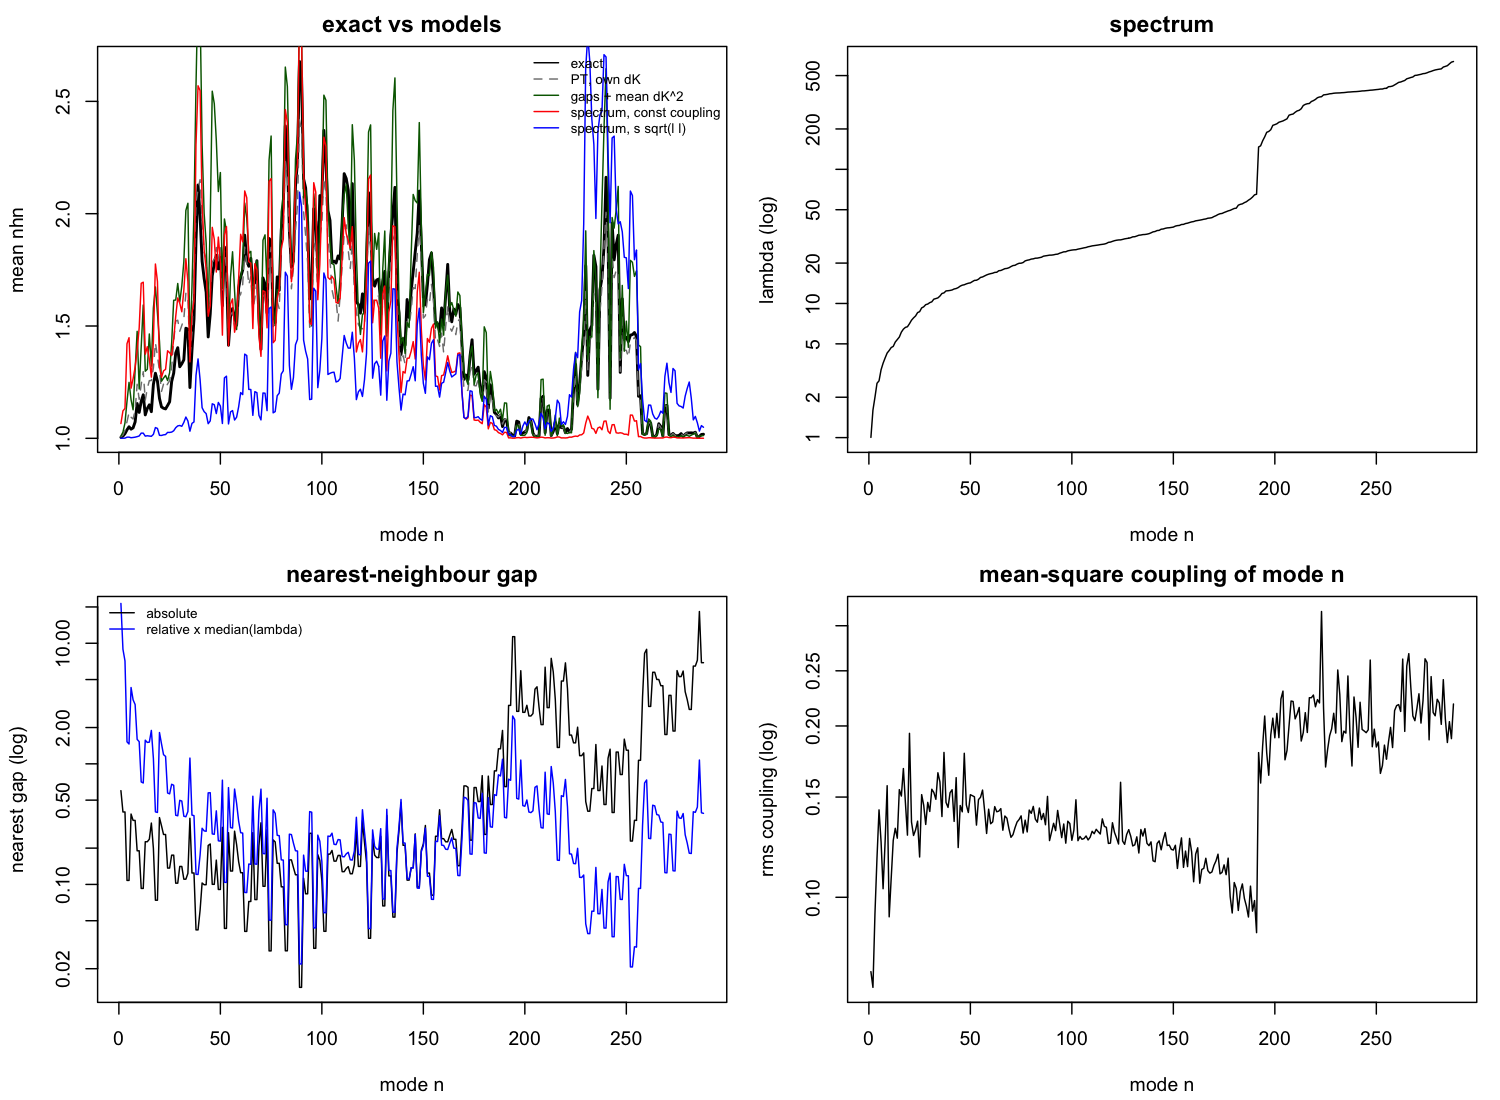
\includegraphics[width=\textwidth]{nhn_explain.png}
\caption{Top left: mean \code{nhn} over the 882 mutants (black) and the models (i), (ii), (iii)
and (v). Top right: the wild type's spectrum. Bottom left: the gap to the nearest eigenvalue,
absolute and relative. Bottom right: the root-mean-square coupling of mode $n$ to the other modes,
over the scan.}
\label{fig:explain}
\end{figure}

\begin{figure}[ht]
\centering
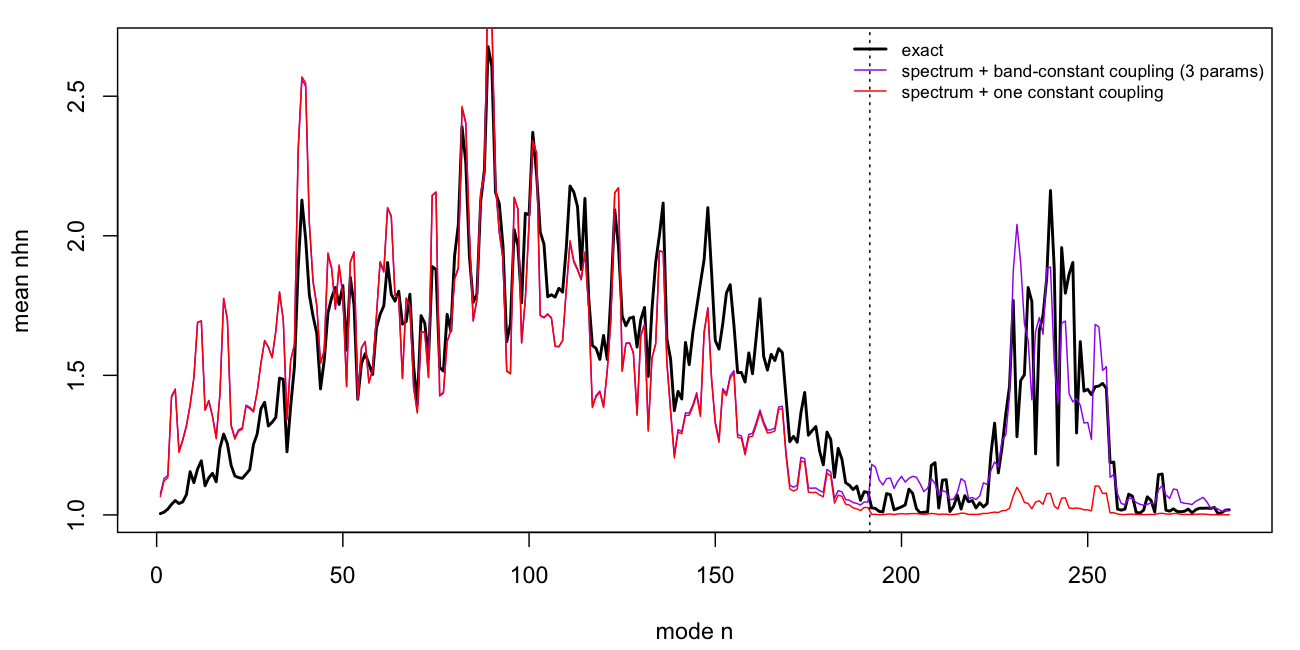
\includegraphics[width=\textwidth]{nhn_bands.png}
\caption{Mean \code{nhn} (black), with model (iv), one coupling scale per pair of bands (purple),
and model (iii), one constant coupling (red). The dotted line marks the band gap.}
\label{fig:bands}
\end{figure}

\paragraph{What the spectrum explains.} With one constant coupling, the model reproduces the fine
structure of the lower band: the peaks of \code{nhn} sit at small gaps. The fitted constant,
0.039, matches the measured rms coupling within the lower band, 0.038; model (iv) fits 0.197 for
the upper band against 0.19 measured. Its cross-band scale, 1.02 against 0.218 measured, is
poorly determined.

\paragraph{What it misses.}
\begin{itemize}
\item The upper band couples about five times more strongly than the lower; with one constant
  coupling its hump disappears (Figure~\ref{fig:bands}).
\item The lowest modes, $n\lesssim35$, are more robust than their gaps predict: their rms
  coupling to the other modes is about half the middle modes', rising over the first $\sim$20
  modes as $\lambda$ goes from 1 to $\sim$10. An unchecked guess at why: soft modes are near-rigid
  motions of domains that barely deform the local springs a mutation perturbs.
\item The model undershoots around $n\approx140$--175; not looked into.
\end{itemize}

So the spectral density accounts for most of the profile, including where its peaks are, but
not all of it: the lowest modes are robust both because of their gaps and because they couple
weakly to mutations, and the second is not a spectral effect.

\section{Open questions}

\begin{itemize}
\item With a single band, \code{model = "anm"}, is the profile a single inverted U?
\item Does the lowest modes' coupling to mutations scale with $\lambda$?
\item How large is the second-order contamination of the two Rayleigh quotients on real mutants?
\item Do these results hold for other proteins, models and ensembles?
\end{itemize}

\end{document}
